% Constructed and checked from the problem; not a geometric proof.
\documentclass[tikz,border=8pt]{standalone}
\begin{document}
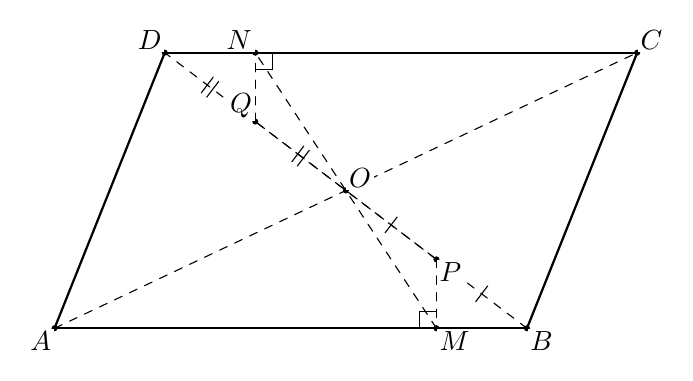
\begin{tikzpicture}[scale=1,line cap=round,line join=round]
\coordinate (p0) at (0,0);
\coordinate (p1) at (6,0);
\coordinate (p2) at (7.4,3.5);
\coordinate (p3) at (1.4,3.5);
\coordinate (p4) at (3.7,1.75);
\coordinate (p5) at (4.85,0.875);
\coordinate (p6) at (2.55,2.625);
\coordinate (p7) at (4.85,0);
\coordinate (p8) at (2.55,3.5);
\draw[thick] (p0) -- (p1);
\draw[thick] (p1) -- (p2);
\draw[thick] (p2) -- (p3);
\draw[thick] (p3) -- (p0);
\draw[dashed] (p0) -- (p2);
\draw[dashed] (p1) -- (p3);
\draw[dashed] (p5) -- (p7);
\draw[dashed] (p6) -- (p8);
\draw[dashed] (p7) -- (p8);
\draw[dashed] (p5) -- (p6);
\draw (4.3511746,1.4126152) -- (4.1988254,1.2123848);
\draw (5.5011746,0.5376152) -- (5.3488254,0.3373848);
\draw (3.0838657,2.0607236) -- (3.236215,2.2609541);
\draw (3.013785,2.1140459) -- (3.1661343,2.3142764);
\draw (1.9338657,2.9357236) -- (2.086215,3.1359541);
\draw (1.863785,2.9890459) -- (2.0161343,3.1892764);
\draw (4.85,0.21386) -- (4.63614,0.21386);
\draw (4.63614,0.21386) -- (4.63614,0);
\draw (2.55,3.28614) -- (2.76386,3.28614);
\draw (2.76386,3.28614) -- (2.76386,3.5);
\fill (p0) circle (1.1pt) node[fill=white,inner sep=1pt,below left] {$A$};
\fill (p1) circle (1.1pt) node[fill=white,inner sep=1pt,below right] {$B$};
\fill (p2) circle (1.1pt) node[fill=white,inner sep=1pt,above right] {$C$};
\fill (p3) circle (1.1pt) node[fill=white,inner sep=1pt,above left] {$D$};
\fill (p4) circle (1.1pt) node[fill=white,inner sep=1pt,above right] {$O$};
\fill (p5) circle (1.1pt) node[fill=white,inner sep=1pt,below right] {$P$};
\fill (p6) circle (1.1pt) node[fill=white,inner sep=1pt,above left] {$Q$};
\fill (p7) circle (1.1pt) node[fill=white,inner sep=1pt,below right] {$M$};
\fill (p8) circle (1.1pt) node[fill=white,inner sep=1pt,above left] {$N$};
\end{tikzpicture}
\end{document}
